\documentclass[12pt]{beamer}
\usepackage{../Estilos/BeamerFC}
\usepackage{../Estilos/ColoresLatex}
\usepackage{courier}
\usepackage{listingsutf8}
\usepackage{listings}
\usepackage{xcolor}
\usepackage{textcomp}
\usepackage{color}
\definecolor{deepblue}{rgb}{0,0,0.5}
\definecolor{brown}{rgb}{0.59, 0.29, 0.0}
\definecolor{OliveGreen}{rgb}{0,0.25,0}
% \usepackage{minted}

\DeclareCaptionFont{white}{\color{white}}
\DeclareCaptionFormat{listing}{\colorbox{gray}{\parbox{0.98\textwidth}{#1#2#3}}}
\captionsetup[lstlisting]{format=listing,labelfont=white,textfont=white}
\renewcommand{\lstlistingname}{Código}


\definecolor{Code}{rgb}{0,0,0}
\definecolor{Keywords}{rgb}{255,0,0}
\definecolor{Strings}{rgb}{255,0,255}
\definecolor{Comments}{rgb}{0,0,255}
\definecolor{Numbers}{rgb}{255,128,0}

\makeatletter

\newif\iffirstchar\firstchartrue
\newif\ifstartedbyadigit
\newif\ifprecededbyequalsign

\newcommand\processletter
{%
  \ifnum\lst@mode=\lst@Pmode%
    \iffirstchar%
        \global\startedbyadigitfalse%
      \fi
      \global\firstcharfalse%
    \fi
}

\newcommand\processdigit
{%
  \ifnum\lst@mode=\lst@Pmode%
      \iffirstchar%
        \global\startedbyadigittrue%
      \fi
      \global\firstcharfalse%
  \fi
}

\lst@AddToHook{OutputOther}%
{%
  \lst@IfLastOtherOneOf{=}
    {\global\precededbyequalsigntrue}
    {}%
}

\lst@AddToHook{Output}%
{%
  \ifprecededbyequalsign%
      \ifstartedbyadigit%
        \def\lst@thestyle{\color{orange}}%
      \fi
    \fi
  \global\firstchartrue%
  \global\startedbyadigitfalse%
  \global\precededbyequalsignfalse%
}

\lstset{ 
language=Python,                % choose the language of the code
basicstyle=\footnotesize\ttfamily,       % the size of the fonts that are used for the code
numbers=left,                   % where to put the line-numbers
numberstyle=\scriptsize,      % the size of the fonts that are used for the line-numbers
stepnumber=1,                   % the step between two line-numbers. If it is 1 each line will be numbered
numbersep=5pt,                  % how far the line-numbers are from the code
backgroundcolor=\color{white},  % choose the background color. You must add \usepackage{color}
showspaces=false,               % show spaces adding particular underscores
showstringspaces=false,         % underline spaces within strings
showtabs=false,                 % show tabs within strings adding particular underscores
frame=single,   		% adds a frame around the code
tabsize=2,  		% sets default tabsize to 2 spaces
captionpos=t,   		% sets the caption-position to bottom
breaklines=true,    	% sets automatic line breaking
breakatwhitespace=false,    % sets if automatic breaks should only happen at whitespace
escapeinside={| |},  % if you want to add a comment within your code
stringstyle =\color{OliveGreen},
otherkeywords={as, np.array, np.concatenate, np.linspace, linspace, interpolate.interp1d, kind, plt.plot, .copy, np.arange, np.cos, np.pi, lw, ls, label, splrep, splev, plt.legend, loc, plt.title, plt.ylim, plt.show, sign, math.ceil, math.log, np.sqrt, np.exp, np.zeros, plt.xlabel, plt.ylabel, plt.xlim, np.identity, random, np.dot, np.outer, np.diagonal },             % Add keywords here
keywordstyle = \color{blue},
commentstyle = \color{darkcerulean},
identifierstyle = \color{black},
literate=%
         {á}{{\'a}}1
         {é}{{\'e}}1
         {í}{{\'i}}1
         {ó}{{\'o}}1
         {ú}{{\'u}}1
%
%keywordstyle=\ttb\color{deepblue}
%fancyvrb = true,
}

\lstdefinestyle{FormattedNumber}{%
    literate={0}{{\textcolor{red}{0}}}{1}%
             {1}{{\textcolor{red}{1}}}{1}%
             {2}{{\textcolor{red}{2}}}{1}%
             {3}{{\textcolor{red}{3}}}{1}%
             {4}{{\textcolor{red}{4}}}{1}%
             {5}{{\textcolor{red}{5}}}{1}%
             {6}{{\textcolor{red}{6}}}{1}%
             {7}{{\textcolor{red}{7}}}{1}%
             {8}{{\textcolor{red}{8}}}{1}%
             {9}{{\textcolor{red}{9}}}{1}%
             {.0}{{\textcolor{red}{.0}}}{2}% Following is to ensure that only periods
             {.1}{{\textcolor{red}{.1}}}{2}% followed by a digit are changed.
             {.2}{{\textcolor{red}{.2}}}{2}%
             {.3}{{\textcolor{red}{.3}}}{2}%
             {.4}{{\textcolor{red}{.4}}}{2}%
             {.5}{{\textcolor{red}{.5}}}{2}%
             {.6}{{\textcolor{red}{.6}}}{2}%
             {.7}{{\textcolor{red}{.7}}}{2}%
             {.8}{{\textcolor{red}{.8}}}{2}%
             {.9}{{\textcolor{red}{.9}}}{2}%
             {\ }{{ }}{1}% handle the space
         ,%
          %mathescape=true
          escapeinside={__}
          }



\usetheme{Dresden}
\usecolortheme{seahorse}
%\useoutertheme{default}
\setbeamercovered{invisible}
% or whatever (possibly just delete it)
\setbeamertemplate{section in toc}[sections numbered]
\setbeamertemplate{subsection in toc}[subsections numbered]
\setbeamertemplate{subsection in toc}{\leavevmode\leftskip=3.2em\rlap{\hskip-2em\inserttocsectionnumber.\inserttocsubsectionnumber}\inserttocsubsection\par}
\setbeamercolor{section in toc}{fg=blue}
\setbeamercolor{subsection in toc}{fg=blue}
\setbeamercolor{frametitle}{fg=blue}
\setbeamertemplate{caption}[numbered]

\setbeamertemplate{footline}
\beamertemplatenavigationsymbolsempty
\setbeamertemplate{headline}{}

\makeatletter
\setbeamercolor{section in foot}{bg=gray!30, fg=black!90!orange}
\setbeamercolor{subsection in foot}{bg=blue!30!yellow, fg=red}
\setbeamertemplate{footline}
{
  \leavevmode%
  \hbox{%
  \begin{beamercolorbox}[wd=.333333\paperwidth,ht=2.25ex,dp=1ex,center]{section in foot}%
    \usebeamerfont{section in foot} \insertsection
  \end{beamercolorbox}}%
  \begin{beamercolorbox}[wd=.333333\paperwidth,ht=2.25ex,dp=1ex,center]{subsection in foot}%
    \usebeamerfont{subsection in foot}  \insertsubsection
  \end{beamercolorbox}%
  \begin{beamercolorbox}[wd=.333333\paperwidth,ht=2.25ex,dp=1ex,right]{date in head/foot}%
    \usebeamerfont{date in head/foot} \insertshortdate{} \hspace*{2em}
    \insertframenumber{} / \inserttotalframenumber \hspace*{2ex} 
  \end{beamercolorbox}}%
  \vskip0pt%
\makeatother 

\makeatletter
\patchcmd{\beamer@sectionintoc}{\vskip1.5em}{\vskip0.8em}{}{}
\makeatother

\usefonttheme{serif}

\title{\large{Integración numérica}}
\subtitle{Tema 2 - Operaciones matemáticas básicas}
\author{M. en C. Gustavo Contreras Mayén}
\date{}

\begin{document}
\maketitle

\section*{Contenido}
\frame{\tableofcontents[currentsection, hideallsubsections]}

\section{Integración numérica}
\frame{\tableofcontents[currentsection, hideothersubsections]}
\subsection{Problema inicial}

\begin{frame}
\frametitle{Problema inicial}
Dada la función $f (x)$, queremos calcular de manera numérica:
\begin{align*}
\scaleint{6ex}_{\bs a}^{b} f (x) \dd{x}
\end{align*}
\end{frame}

\section{Introducción}
\frame{\tableofcontents[currentsection, hideothersubsections]}
\subsection{Base de la integración numérica}

\begin{frame}
\frametitle{Introducción}
La integración numérica (también conocida como \textcolor{blue}{cuadratura}) es un procedimiento con mayor precisión que la diferenciación numérica.
\end{frame}
\begin{frame}
\frametitle{Introducción}
La cuadratura aproxima la integral definida:
\pause
\begin{align*}
\scaleint{6ex}_{\bs a}^{b} f (x) \dd{x}
\end{align*}
mediante la suma:
\begin{align*}
I = \nsum_{i=0}^{n} A_{i} \, f (x_{i})
\end{align*}
\fontsize{12}{12}\selectfont
donde las \textcolor{ao}{abscisas nodales} $x_{i}$ \pause y los \textcolor{amethyst}{pesos} $A_{i}$ dependen de una regla en particular usada para la cuadratura.
\end{frame}
\begin{frame}
\frametitle{Clasificación de las cuadraturas}
Todas las reglas de cuadratura se dividen en dos grupos:
\pause
\setbeamercolor{item projected}{bg=amber,fg=arsenic}
\setbeamertemplate{enumerate items}{%
\usebeamercolor[bg]{item projected}%
\raisebox{1.5pt}{\colorbox{bg}{\color{fg}\footnotesize\insertenumlabel}}%
}
\begin{enumerate}[<+->]
\item Fórmulas de \textcolor{blue-violet}{Newton-Cotes}.
\item Fórmulas de \textcolor{americanrose}{Cuadraturas Gaussianas}.
\end{enumerate}
\end{frame}

\section{Fórmulas de Newton-Cotes}
\frame{\tableofcontents[currentsection, hideothersubsections]}
\subsection{Definición de las fórmulas}

\begin{frame}
\frametitle{Fórmulas de Newton-Cotes}
Estas fórmulas se caracterizan por usar un \textcolor{blue(pigment)}{espaciamiento uniforme y constante en las abscisas}, \pause aquí se consideran los \textcolor{blush}{métodos del trapecio} y la \textcolor{bole}{regla de Simpson}.
\end{frame}
\begin{frame}
\frametitle{Fórmulas de Newton-Cotes}
Son útiles si la $f (x)$ se ha evaluado en intervalos iguales.
\\
\bigskip
\pause
Las fórmulas Newton-Cotes se basan en una \textbf{interpolación local}, se requiere de una porción del dominio para ajustarla al polinomio.
\end{frame}
\begin{frame}
\frametitle{Fórmulas de Newton-Cotes}
Consideremos la integral definida:
\pause
\begin{align*}
\scaleint{6ex}_{\bs a}^{b} f (x)\dd{x}
\end{align*}
\pause
Dividimos el intervalo de integración $[a, b]$ en $n$ intervalos de igual longitud $h = (b - a)/n$, y hacemos que las abscisas sean $x_{0},x_{1}, \ldots, x_{n}$.
\end{frame}
\begin{frame}
\frametitle{Aproximación polinomial de $f (x)$}
\begin{figure}
    \centering
    \includestandalone[scale=0.95]{Figuras/integracion_01}
\end{figure}
\end{frame}
\begin{frame}
\frametitle{Aproximación polinomial de $f (x)$}
Ahora aproximamos $f (x)$ con un polinomio de orden $n$ que intersecta todos los nodos.
\\
\bigskip
\pause
Recordemos que la expresión para el polinomio de Lagrange es:
\begin{align*}
P_{n} (x) = \nsum_{i=0}^{n} f (x_{i}) \, \mathcal{L}_{i} (x)
\end{align*}
donde $\mathcal{L}_{i} (x)$ son las funciones cardinales definidas en el tema de interpolación. 
\end{frame}
\begin{frame}
\frametitle{Aproximación polinomial de $f (x)$}
Por tanto, un aproximación a la integral es:
\pause
\begin{eqnarray*}
\begin{aligned}
I &= \scaleint{6ex}_{\bs a}^{b} P_{n} (x) \dd{x} = \nsum_{i=0}^{n} \left[ f (x_{i}) \scaleint{6ex}_{\bs a}^{b} \mathcal{L}_{i} (x) \dd{x} \right] = \\[0.5em] \pause 
&= \sum_{i=0}^{n} A_{i} f (x_{i})
\end{aligned}
\end{eqnarray*}
\pause
donde:
\begin{align*}
A_{i} = \scaleint{6ex}_{\bs a}^{b} \mathcal{L}_{i} \dd{x}, \hspace{1cm} i = 0, 1, \ldots, n
\end{align*}
\end{frame}
\begin{frame}
\frametitle{Fórmulas de Newton-Cotes}
Las ecuaciones:
\pause
\begin{eqnarray*}
\begin{aligned}
I &= \scaleint{6ex}_{\bs a}^{b} P_{n} (x) \dd{x} = \nsum_{i=0}^{n} \left[ f (x_{i}) \scaleint{6ex}_{\bs a}^{b} \mathcal{L}_{i}(x) \dd{x} \right] = \\[0.5em] \pause
&= \sum_{i=0}^{n} A_{i} f (x_{i})
\end{aligned}
\end{eqnarray*}
\pause
se conocen como las fórmulas de Newton-Cotes.
\end{frame}
\begin{frame}
\frametitle{Fórmulas de Newton-Cotes}
Siendo los casos:
\pause
\setbeamercolor{item projected}{bg=buff,fg=carmine}
\setbeamertemplate{enumerate items}{%
\usebeamercolor[bg]{item projected}%
\raisebox{1.5pt}{\colorbox{bg}{\color{fg}\footnotesize\insertenumlabel}}%
}
\begin{enumerate}[<+->]
\item $n = 1$, Regla del trapecio.
\item $n = 2$, Regla de Simpson.
\item $n = 3$, Regla de Simpson de $3/8$.
\end{enumerate}
\end{frame}
\begin{frame}
\frametitle{Fórmulas de Newton-Cotes}
La más importante es la regla del trapecio, ya que se puede combinar con la \textit{extrapolación de Richardson}, en un algoritmo eficiente llamado: \textcolor{cobalt}{Integración de Romberg}.
\end{frame}

\subsection{Regla del trapecio}

\begin{frame}
\frametitle{Regla del trapecio}
\begin{figure}
	\centering
	\includestandalone{Figuras/integracion_02}
\end{figure}
\end{frame}
\begin{frame}
\frametitle{Regla del trapecio}
Si $n = 1$ (un bloque), \pause tenemos que $l_{0} = (x - x_{1})/(x_{0} - x_{1})= (x - b)/h$ por tanto:
\pause
\begin{align*}
A_{0} = \dfrac{1}{h} \scaleint{6ex}_{\bs a}^{b} (x - b) \dd{x} = \dfrac{1}{2 \, h} (b - a)^{2} = \dfrac{h}{2}
\end{align*}
\end{frame}
\begin{frame}
\frametitle{Regla del trapecio}
Para $l_{1} = (x - x_{0})/(x_{1} - x_{0}) = (x - a)/h$ tenemos:
\pause
\begin{align*}
A_{1} = \dfrac{1}{h} \scaleint{6ex}_{\bs a}^{b} (x - a) \dd{x} = \dfrac{1}{2h} (b-a)^{2}= \dfrac{h}{2}
\end{align*}
Sustituyendo las funciones cardinales:
\pause
\begin{align*}
I = \left[ f (a) + f (b) \right] \, \dfrac{h}{2}
\end{align*}
\end{frame}
\begin{frame}
\frametitle{Regla del trapecio}
Que resulta ser la regla del trapecio, y representa el área del trapecio de la figura:
\begin{figure}
	\centering
	\includestandalone[scale=1]{Figuras/integracion_02}
\end{figure}
\end{frame}

\subsection{Error en la regla del trapecio}

\begin{frame}
\frametitle{Error en la regla del trapecio}
El error por la aproximación viene dado por:
\pause
\begin{align*}
E = \scaleint{6ex}_{\bs a}^{b} f (x) \dd{x} - I
\end{align*}
que es diferencia entre el área debajo de la curva de $f (x)$ y el la integral obtenida. 
\end{frame}
\begin{frame}
\frametitle{Error por la interpolación}
Integrando el error de interpolación:
\pause
\begin{eqnarray*}
\begin{aligned}
E &= \dfrac{1}{2!} \: \scaleint{6ex}_{\bs a}^{b} (x - x_{0})(x - x_{1}) \: \sderivada{f} (\xi) \: \dd{x}  \\ \pause
&= \dfrac{1}{2} \: \sderivada{f} (\xi) \: \scaleint{6ex}_{\bs a}^{b} (x - a)(x - b) \: \dd{x} = \\ \pause
&= -\dfrac{1}{12}(b - a)^{3} \sderivada{f} (\xi) \\ \pause
&= -\dfrac{h^{3}}{12} \: \sderivada{f} (\xi)
\end{aligned}
\end{eqnarray*}
\end{frame}

\subsection{Regla extendida del trapecio}

\begin{frame}
\frametitle{Regla extendida del trapecio}
En la práctica la regla del trapecio se usa con una división en el dominio. \pause La siguiente figura muestra la región $[a, b]$ dividida en $n$ bloques, de longitud $h$.
\pause
\begin{figure}
	\centering
	\includestandalone[scale=1.2]{Figuras/integracion_03}
\end{figure}
\end{frame}
\begin{frame}
\frametitle{Regla extendida del trapecio}
La función $f (x)$ se integrará con una aproximación lineal en cada panel. 
\\
\bigskip
\pause
De la regla del trapecio, sabemos que para el i-ésimo panel:
\pause
\begin{align*}
I_{i} = [ f (x_{i}) + f (x_{i+1}) ] \, \dfrac{h}{2}
\end{align*}
\end{frame}
\begin{frame}
\frametitle{Regla extendida del trapecio}
El área total queda representada por la integral:
\pause
\begin{align*}
I &\simeq \nsum_{i=0}^{n-1} \bigg[ f (x_{0}) + 2 \, f (x_{1}) + 2 \, f (x_{2}) + \ldots + \\
&+ 2 \, f (x_{n-1}) + f (x_{n}) \bigg] \, \dfrac{h}{2}
\end{align*}
que es la regla del extendida del trapecio.
\end{frame}

\subsection{Regla recursiva del trapecio}

\begin{frame}
\frametitle{Regla recursiva del trapecio}
Sea $I_{k}$ la integral evaluada con la regla compuesta del trapecio, usando $2^{k-1}$ bloques. \pause Con la notación $H = b - a$, de la regla compuesta del trapecio, para $k = 1, 2, 3$:
\begin{align*}
k &= 1 \text{ (1 bloque) }: \\
I_{1} &= \bigg[f (a) + f (b) \bigg] \dfrac{H}{2}
\end{align*}
\end{frame}
\begin{frame}
\frametitle{Regla recursiva del trapecio}
\begin{eqnarray*}
\begin{aligned}
k &= 2 \text{ (2 bloques) }: \\ \pause
I_{2} &= \left[ f (a) + 2 \: f \left( a + \dfrac{H}{2} \right) + f (b) \right] \dfrac{H}{4} \\ \pause
&= \dfrac{1}{2} \: I_{1} + f \left( a + \dfrac{H}{2} \right) \: \dfrac{H}{2}
\end{aligned}
\end{eqnarray*}
\end{frame}
\begin{frame}
\frametitle{Regla recursiva del trapecio}
\begin{eqnarray*}
\begin{aligned}
k &= 3 \text{ (4 bloques) }: \\ \pause
I_{3} &= \left[ f (a) + 2 \: f \left(a + \dfrac{H}{4} \right) + 2 \: f \left( a + \dfrac{H}{2} \right) + \right.\\
&+ \left. 2 \: f \left( a + \dfrac{3 \: H}{4} \right) + f (b) \right] \dfrac{H}{8} \\ \pause
&= \dfrac{1}{2} \: I_{2} \left[ f \left(a + \dfrac{H}{4} \right) + f \left( a + \dfrac{3 \: H}{4}\right) \right] \: \dfrac{H}{4}
\end{aligned}
\end{eqnarray*}
\end{frame}
\begin{frame}
\frametitle{Regla recursiva del trapecio}
Para un $k > 1$ arbitrario, tenemos que:
\pause
\begin{align*}
I_{k} = \dfrac{1}{2} \: I_{k - 1} + \dfrac{H}{2^{k - 1}} \nsum_{i = 1}^{2^{k - 2}} \: f \left[ a + \dfrac{(2 \: i - 1)H}{2^{k - 1}} \right], \hspace{0.4cm} k = 2, 3, \ldots
\end{align*}
\pause
Otra forma de la misma ecuación es:
\pause
\begin{align*}
I(h) = \dfrac{1}{2} \: I(2 \: h) + h \sum f (_{\text{nuevo}})
\end{align*}
\end{frame}

\subsection{Ejercicio}

\begin{frame}
\frametitle{Ejercicio}
El cuerpo de revolución que se muestra en la siguiente figura, se obtiene al girar la curva dada por:
\begin{align*}
y = 1 + \left( \dfrac{x}{2} \right)^{2}, \hspace{0.5cm} 0 \leq x \leq 2
\end{align*}
en torno al eje $x$.
\end{frame}
\begin{frame}
\frametitle{Figura para el ejercicio}
\begin{figure}
	\centering
	\includestandalone{Figuras/integracion_04}
\end{figure}
\end{frame}
\begin{frame}
\frametitle{Ejercicio}
\setbeamercolor{item projected}{bg=brightgreen,fg=bole}
\setbeamertemplate{enumerate items}{%
\usebeamercolor[bg]{item projected}%
\raisebox{1.5pt}{\colorbox{bg}{\color{fg}\footnotesize\insertenumlabel}}%
}
\begin{enumerate}[<+->]
\item Calcula el volumen del sólido, usando la regla extendida del trapecio con $N = 2, 4, 8, 16, 32, 64, 128$.
\item Evalúa el error para cada $N$. El valor exacto del volumen es es $I = 11.7286$.
\end{enumerate}
\end{frame}
\begin{frame}
\frametitle{Resolviendo el problema}
Hay que definir inicialmente la función que queremos integrar, por tanto:
\pause
\begin{align*}
I = \scaleint{6ex}_{\bs a}^{b} f (x) \dd{x}
\end{align*}
\pause
donde:
\begin{align*}
f (x) = \pi  \bigg[ 1 + \left( \dfrac{x}{2} \right)^{2} \bigg]^{2}
\end{align*}
\end{frame}
\begin{frame}
\frametitle{Gráfica de la función}
Si graficamos la función anterior, tendremos:
\begin{figure}
    \centering
    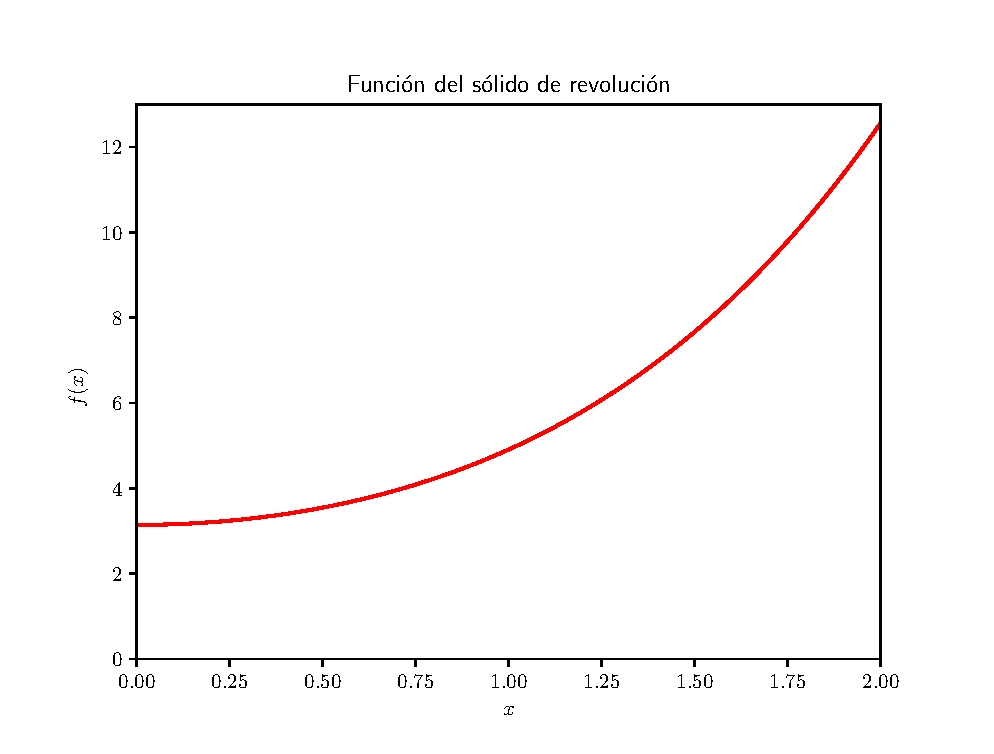
\includegraphics[scale=0.5]{Imagenes/integracion_ejercicio_solido_rev_01.eps}
\end{figure}
\end{frame}
\begin{frame}
\frametitle{Un módulo para funciones de integración}
Las funciones que ocuparemos para la parte de integración quedarán dentro del módulo \funcionazul{moduloIntegracion}, para hacer las correspondientes llamadas en los archivos de los ejercicios.
\end{frame}
\begin{frame}[allowframebreaks, fragile]
\frametitle{Código para el método del trapecio}
\begin{lstlisting}[caption=Código para la función trapecios]
def trapecios(f, a, b, n):
    h = (b - a)/float(n)
    x = a
    suma = f(a)
    
    for i in range(1, n):
       x = x + h
       suma = suma + 2 * f(x)
    
    suma = suma + f(b)
    
    return h * (suma * 0.5)
\end{lstlisting}
\end{frame}
\begin{frame}[fragile]
\frametitle{Declaramos la función}
\begin{lstlisting}[caption=Código para la función f (x)]
import numpy as np

def f(x):
    return np.pi * (1 + (x/2)**2)**2
\end{lstlisting}
    \end{frame}
\begin{frame}[fragile]
\frametitle{Ejercicio completo}
\begin{lstlisting}[caption=Completamos el código y evaluamos el error]
paneles = [2, 4, 8, 16, 32, 64, 128]

for n in paneles:
    h = 2./n
    integral = trapecios(f, 0, 2, n)
    error = error_rel(exacta, integral)
    print(n, h, integral, error)
\end{lstlisting}
\end{frame}
\begin{frame}
\frametitle{Observación}
Nótese que la manera en que incrementamos el valor de $N$, es más dinámica: \pause si aumentamos el número de elementos, tendríamos que ajustar \enquote{a mano} el contenido de una lista.
\\
\bigskip
\pause 
Hacerlo con un incremento en el exponente, nos permite entonces, manejar cualquier cambio en el número de elementos sin problema ni ajustes manuales.
\end{frame}
\begin{frame}
\frametitle{Resultados en una tabla}
\begin{table}
\centering
\renewcommand{\arraystretch}{0.9}
\begin{tabular}{r | c | c | c} \hline
n & h & Integral & Error rel \\ \hline
$2$ & $1.00000$ & $12.762720155$ & $8.81708094e-02$ \\ \hline
$4$ & $0.50000$ & $11.989593838$ & $2.22527700e-02$ \\ \hline
$8$ & $0.25000$ & $11.794011288$ & $5.57707550e-03$ \\ \hline
$16$ & $0.12500$ & $11.744971839$ & $1.39589033e-03$ \\ \hline
$32$ & $0.06250$ & $11.732702989$ & $3.49827695e-04$ \\ \hline
$64$ & $0.03125$ & $11.729635215$ & $8.82641387e-05$ \\ \hline
$128$ & $0.01562$ & $11.728868236$ & $2.28702562e-05$ \\ \hline
\end{tabular}
\end{table}
\end{frame}
\begin{frame}
\frametitle{Sobre el error relativo}
De la tabla anterior, encontramos que el error relativo va disminuyendo de manera proporcional con $h^{2}$.
\end{frame}
\begin{frame}
\frametitle{Gráfica esquemática}
La siguiente gráfica se hizo con \funcionazul{matplotlib.pyplot} con el fin de ilustrar el proceso de integración con el método del trapecio.
\\
\bigskip
\pause
Se han utilizado otras funciones que nos permiten \enquote{dibujar} los bloques para los trapecios.
\end{frame}
\begin{frame}
\frametitle{Gráfica esquemática}
\begin{figure}
    \centering
    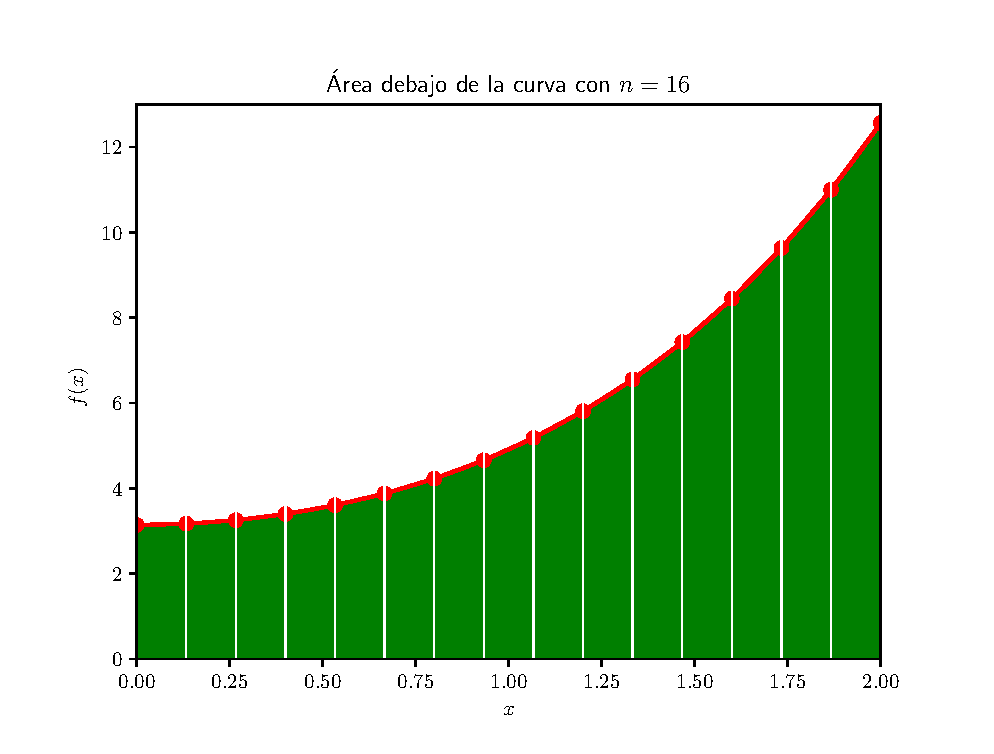
\includegraphics[scale=0.55]{Imagenes/integracion_ejercicio_solido_rev_02.eps}
\end{figure}
\end{frame}

\section{Librería Scipy}
\frame{\tableofcontents[currentsection, hideothersubsections]}
\subsection{¿Qué es scipy?}

\begin{frame}
\frametitle{Librería Scipy}
\funcionazul{SciPy} (Scientific Python) es una librería matemática con funciones que extienden la librería \funcionazul{numpy} para \python.
\\
\bigskip
\pause
De tal manera que se le proporciona al usuario un poder significativo mediante el uso de comandos de alto nivel y clases, para la manipulación y visualización de datos.
\end{frame}

\subsection{Organización de Scipy}

\begin{frame}
\frametitle{Organización de Scipy}
La librería \funcionazul{SciPy} está organizada en sub-paquetes que cubren diferentes áreas de computación científica. Estos se resumen en la siguiente tabla:
\end{frame}
\begin{frame}
\frametitle{Organización de Scipy}
\fontsize{12}{12}\selectfont
\begin{table}
\renewcommand{\arraystretch}{0.9}
\begin{tabular}{l | l}
	Subpaquete	&	Descripción \\ \hline
	cluster		&	Algortimos para clusters \\ \hline
	constants	&	Constantes físicas y matemáticas \\ \hline
	fftpack 	&	Rutinas para la Transformada Rápida de Fourier \\ \hline
	integrate	&	Integración y EDO \\ \hline
	interpolate	&	Interpolación y uso de splines \\ \hline
	io			&	Rutinas de entrada y salida
\end{tabular}
\end{table}
\end{frame}
\begin{frame}
\frametitle{Organización de Scipy}
\fontsize{12}{12}\selectfont
\begin{table}
\renewcommand{\arraystretch}{0.9}
\begin{tabular}{l | l}
	Subpaquete	&	Descripción \\ \hline
	linalg		&	Algebra lineal \\ \hline
	ndimage		&	Procesamiento N-dimensional de imágenes \\ \hline
	odr			&	Regresión de distancias ortogonales \\ \hline
	optimize	&	Optimización y rutinas para encontrar raíces \\ \hline
	signal		&	Procesamiento de señales \\ \hline
\end{tabular}
\end{table}
\end{frame}
\begin{frame}
\frametitle{Organización de Scipy}
\fontsize{12}{12}\selectfont
\begin{table}
\renewcommand{\arraystretch}{0.9}
\begin{tabular}{l | l}
    sparse		&	Matrices sparse y rutinas asociadas \\ \hline
    spatial		&	Estructura de datos espaciales \\ \hline
    special		&	Funciones especiales \\ \hline
    stats		&	Distribuciones estadísticas \\ \hline
    weave		&	Integración con C/C++
\end{tabular}
\end{table}
\end{frame}
    
\subsection{\texttt{scipy.integrate}}

\begin{frame}
\frametitle{Integración (\texttt{scipy.integrate})}
El subpaquete \funcionazul{scipy.integrate} proporciona varias técnicas de integración.
\pause
\fontsize{12}{12}\selectfont
\begin{table}
\renewcommand{\arraystretch}{0.9}
\begin{tabular}{l | p{8cm}}
quad 		& Integración en general. \\ \hline
dblquad 	& Integración doble en general. \\ \hline
tplquad 	& Integración triple en general. \\ \hline
fixed-quad 	& Integración de f (x) usando cuadraturas gaussianas de orden $n$. \\ \hline
quadrature 	& Integra con tolerancia dada usando cuadratura gaussiana. \\ \hline
romberg 	& Integra una función mediante la integración de Romberg.
\end{tabular}
\end{table}
\end{frame}
\begin{frame}[fragile]
\frametitle{Usando \funcionazul{integrate.quad}}
Para comparar el resultado que nos devuelve la función \funcionazul{scipy.integrate.quad}, veamos cómo implementar la solución del problema del sólido de revolución.
\end{frame}
\begin{frame}[fragile]
\frametitle{Usando \funcionazul{integrate.quad}}
\begin{lstlisting}[caption=Integración con scipy]
from numpy import pi
from scipy.integrate import quad

def f(x):
    return pi*(1 + (x/2)**2)**2
   
print(quad(f, 0, 2))
\end{lstlisting}
\pause
El resultado que nos devuelve es: $(11.728612573401893, 1.302137572589889e-13)$.
\end{frame}
\begin{frame}[fragile]
\frametitle{Usando \funcionazul{integrate.quad}}
El \textcolor{burntumber}{primer valor es el valor de la integral}, mientras que el \textcolor{carnelian}{segundo valor es el error} asociado al algoritmo que usa \funcionazul{integrate.quad}, para que no lo reporte en el resultado, basta con indicar que queremos sólo el primer elemento de la lista:
\\
\bigskip
\pause
\verb|print(quad(f, 0, 2)[0])|
\end{frame}

\section{Reglas de Simpson}
\frame{\tableofcontents[currentsection, hideothersubsections]}
\subsection{Regla de \texorpdfstring{$1/3$}{1/3} de Simpson}

\begin{frame}
\frametitle{Regla de $1/3$ de Simpson}
La regla de $1/3$ de Simpson se obtiene de las fórmulas de Newton-Cotes con $n = 2$, \pause es decir, haciendo una interpolación con una parábola a través de tres nodos
\end{frame}
\begin{frame}
\frametitle{Regla de $1/3$ de Simpson}
Como se muestra en la siguiente figura:
\begin{figure}
	\centering
	\includestandalone[scale=0.9]{Figuras/integracion_05}
\end{figure}
\end{frame}
\begin{frame}
\frametitle{Regla de $1/3$ de Simpson}
\begin{figure}
	\centering
	\includestandalone[scale=0.9]{Figuras/integracion_05}
\end{figure}
El área debajo de la curva representa una aproximación a la integral $\scaleint{6ex}_{\bs a}^{b} f (x) \dd{x}$.
\end{frame}
\begin{frame}
\frametitle{Regla de $1/3$ de Simpson}
Es decir:
\begin{align*}
\scaleint{6ex}_{\bs a}^{b} f (x) \simeq I = \left[ f (a) + 4 \: f \left( \dfrac{a + b}{2} \right) + f (b) \right] \: \dfrac{h}{3}
\end{align*}
\end{frame}

\subsection{Regla compuesta de \texorpdfstring{$1/3$}{1/3} de Simpson}

\begin{frame}
\frametitle{Regla compuesta de $1/3$ de Simpson}
Para obtener la regla compuesta de $1/3$ de Simpson, se divide el intervalo de integración $[a, b]$ en $n$ bloques ($n$ par) de ancho $h = (b - a)/n$
\end{frame}
\begin{frame}
\frametitle{Regla compuesta de $1/3$ de Simpson}
\begin{figure}
	\centering
	\includestandalone[scale=1]{Figuras/integracion_06}
\end{figure}
\end{frame}
\begin{frame}
\frametitle{Regla compuesta de $1/3$ de Simpson}
Aplicando la fórmula anterior a dos bloques adyacentes, tenemos:
\pause
\begin{align*}
\scaleint{6ex}_{\bs x_{i}}^{x_{i + 2}} \: f (x) \: \dd{x} \simeq \left[ f (x_{i}) + 4 \: f (x_{i + 1}) + f (x_{i + 2}) \right] \: \dfrac{h}{3} 
\end{align*}
sustituyendo la ecuación en todo el intervalo:
\pause
\begin{align*}
\scaleint{6ex}_{\bs a}^{b} \: f (x) \: \dd{x} = \scaleint{6ex}_{\bs x_{0}}^{x_{m}} \: f (x) \: \dd{x} = \nsum_{i = 0, 2, \ldots}^{n} \left[ \scaleint{6ex}_{\bs x_{i}}^{x_{i + 2}} \: f (x) \: \dd{x} \right]
\end{align*}
\end{frame}
\begin{frame}
\frametitle{Regla compuesta de $1/3$ de Simpson}
Por lo que la aproximación a la integral resulta ser:
\pause
\begin{eqnarray*}
\begin{aligned}
\scaleint{6ex}_{\bs a}^{b} f (x) \dd{x} \simeq I = \left[ f (x_{0}) + 4 \: f (x_{1}) + 2 \: f (x_{2}) + \ldots  \right. \\
\left. \ldots + 2 \: f (x_{n-2}) + 4 \: f (x_{n - 1}) + f (x_{n}) \right] \: \dfrac{h}{3}
\end{aligned}
\end{eqnarray*}
\pause
y es quizás el método más conocido de integración numérica. 
\end{frame}
\begin{frame}
\frametitle{Regla compuesta de $1/3$ de Simpson}
Aunque su reputación es algo inmerecido, ya que la regla del trapecio es más robusta, y la integración de Romberg es más eficiente.
\end{frame}
\begin{frame}
\frametitle{El error en la regla de $1/3$ de Simpson}
El error en la regla compuesta de Simpson viene dado por:
\pause
\begin{align*}
E = \dfrac{(b - a) \, h^{4}}{180} \: f^{(4)} (\xi)
\end{align*}
de donde inferimos que la integral obtenida por el método, es exacta si el polinomio es de grado tres o menor.
\end{frame}

\subsection{Regla de \texorpdfstring{$3/8$}{3/8} de Simpson}

\begin{frame}
\frametitle{Regla de $3/8$ de Simpson}
La regla de $1/3$ de Simpson necesita que el número de bloques $n$ sea par.
\\
\bigskip
\pause
Si la condición no se cumple, podemos integrar sobre los primeros (o últimos) tres bloques con la regla de $3/8$ de Simpson:
\pause
\begin{align*}
I = \bigg[ f (x_{0}) + 3 \: f (x_{1}) + 3 \: f (x_{2}) + f (x_{3}) \bigg] \dfrac{3 \: h}{8}
\end{align*}
y aplicar la regla de $1/3$ de Simpson en los bloques restantes.
\end{frame}
\begin{frame}
\frametitle{Ejercicio 2}
Estimar la integral:
\begin{align*}
\scaleint{6ex}_{\bs 0}^{2.5} f (x) \dd{x}
\end{align*}
a partir de los siguientes datos:
\pause
\fontsize{12}{12}\selectfont
\begin{center}
\begin{tabular}{c | c | c | c | c | c | c}
\hline
$x$ & $0$ & $0.5$ & $1.0$ & $1.5$ & $2.0$ & $2.5$ \\ \hline
$f (x)$ & $1.5000$ & $2.0000$ & $2.0000$ & $1.6364$ & $1.25000$ & $0.9565$ \\ \hline
\end{tabular}
\end{center}
\end{frame}
\begin{frame}
\frametitle{Gráfica de los puntos tabulados}
\begin{figure}
	\centering
	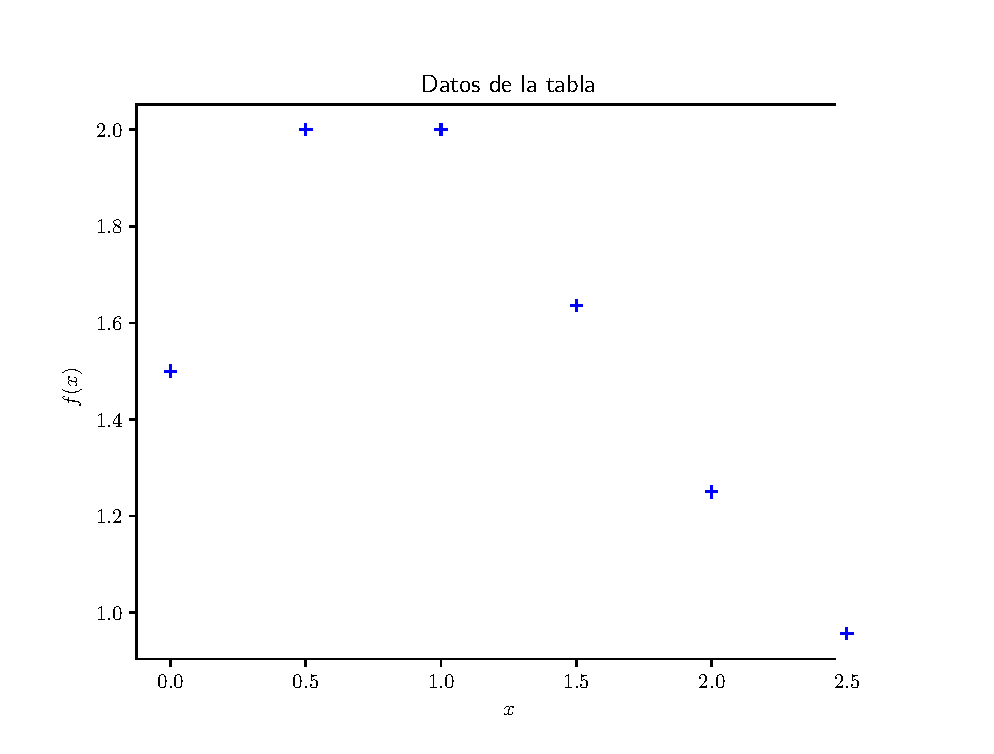
\includegraphics[scale=0.55]{Imagenes/integracion_ejercicio_puntos_01.eps}
\end{figure}
\end{frame}
\begin{frame}
\frametitle{Solución}
Usaremos las reglas de Simpson:
\pause
\setbeamercolor{item projected}{bg=cobalt,fg=columbiablue}
\setbeamertemplate{enumerate items}{%
\usebeamercolor[bg]{item projected}%
\raisebox{1.5pt}{\colorbox{bg}{\color{fg}\footnotesize\insertenumlabel}}%
}
\begin{enumerate}[<+->]
\item Dado que el número de bloques es impar, calculamos la integral sobre los primeros tres bloques con la regla $3/8$ de Simpson.
\item Usamos la regla de $1/3$ de Simpson en los dos últimos bloques.
\end{enumerate}
\end{frame}
\begin{frame}
\frametitle{Solución}
Es decir:
\pause
\begin{eqnarray*}
\begin{aligned}
I &= [f (0) + 3 \, f (0.5) + 3 \, f(1.0) + f \, (1.5)]\dfrac{3 \, (0.5)}{8} \\ \pause
&+ [ f (1.5) + 4 \, f (2.0) + f (2.5)] \dfrac{0.5}{3} \\ \pause
&= 2.8381 + 1.2655 = 4.1036
\end{aligned}
\end{eqnarray*}
\end{frame}
\begin{frame}
\frametitle{Código para resolver el ejercicio}
Al igual que en el caso de diferenciación numérica, las reglas que hemos definido suponen que contamos con una expresión para la función que queremos integrar.
\\
\bigskip
\pause
Por lo que debemos de ajustar el código para manejar pares de puntos $(x_{i}, f (x_{i}))$.
\end{frame}
\begin{frame}[allowframebreaks, fragile]
\frametitle{Regla de Simpson $1/3$ para puntos}
\begin{lstlisting}[caption=Regla de Simpson 1/3 para obtener la integral con pares de puntos]
def simpson13puntos(f, x0, n, h):
	# n debe ser par
	n = n - n%2

	if n<=0: n = 1

	x = x0
	suma = 0

	for j in range(int(n/2)):
		suma += f[0] + 4. * f[1] + f[2]
		x += 2 * h

	return (h/3.) * suma
\end{lstlisting}
\end{frame}
\begin{frame}[allowframebreaks, fragile]
\frametitle{Código para la regla de Simpson 3/8}
\begin{lstlisting}[caption=Regla de Simpson de 3/8 para obtener la integral por pares de puntos]
def simpson38puntos(f, n, h):
	n = n - n%3

	if n <=0: n = 1

	suma = 0
	for j in range(int(n/3)):
		suma += f[0] + 3 * (f[1] + f[2]) + f[3]

	return (3. * h/8) * suma
\end{lstlisting}
\end{frame}
\begin{frame}[allowframebreaks, fragile]
\frametitle{Código completo}
\begin{lstlisting}[caption=Código completo  para el ejercicio]
from moduloIntegracion import simpson38puntos, simpson13puntos

x = [0, 0.5, 1.0, 1.5, 2.0, 2.5]
fx = [1.5000, 2.0000, 2.0000, 1.6364, 1.25000, 0.9565]

print(fx[:4])
print(fx[3:])

integral1 = simpson38puntos(fx[:4], 4, 0.5)
integral2 = simpson13puntos(fx[3:], fx[-3], 3, 0.5)

print('Valor de la integral por la  regla de 3/8 de Simpson = {0:1.6f}'.format(integral1))
print('\nValor de la integral por la  regla de 1/3 de Simpson = {0:1.6f}'.format(integral2))

print('\nValor de la integral = {0:1.6f}'.format(integral1 + integral2))
\end{lstlisting}
\end{frame}
\begin{frame}
\frametitle{Resultado}
Luego de ejecutar el código, se obtiene el valor de la integral para los puntos de la tabla. \pause $ I = 4.103558$
\\
\bigskip
\pause
Mostramos a continuación una gráfica esquemática del procedimiento que realizamos.
\end{frame}
\begin{frame}
\frametitle{Gráfica con las reglas de Simpson}
\begin{figure}
	\centering
	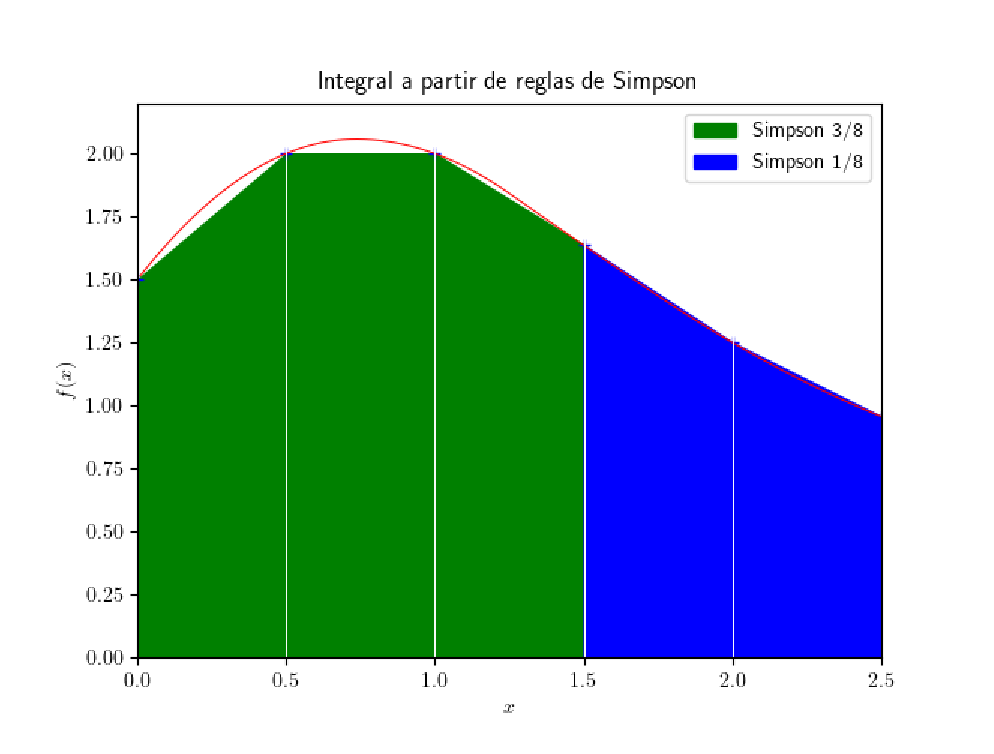
\includegraphics[scale=0.55]{Imagenes/integracion_ejercicio_puntos_02.eps}
\end{figure}
\end{frame}

\subsection{Ejercicio a cuenta}

\begin{frame}
\frametitle{\textbf{Ejercicio a cuenta}}
Un automóvil recorre una pista de carreras en $84$ segundos. Su velocidad en cada intervalo de $4$ segundos se determina mediante una pistola de radar y está dada en pies/segundo, desde el principio del recorrido por los datos de la siguiente tabla:
\end{frame}
\begin{frame}
\frametitle{Tabla de datos de tiempo y velocidad}
\begin{table}
\centering
\begin{tabular}{|*{8}{p{0.7cm}|}} \hline
$t$ & $0$ & $6$ & $12$ & $18$ & $24$ & $30$ & $36$ \\ \hline
$v$ & $124$ & $134$ & $148$ & $156$ & $147$ & $133$ & $121$ \\ \hline
\end{tabular}
\end{table}
\begin{table}
\centering
\begin{tabular}{|*{9}{p{0.7cm}|}} \hline
$t$ & $42$ & $48$ & $54$ & $60$ & $66$ & $72$ & $78$ & $84$ \\ \hline
$v$ & $109$ & $99$ & $85$ & $78$ & $89$ & $104$ & $116$ & $123$ \\ \hline
\end{tabular}
\end{table}
¿Cuál es la longitud de la pista (en metros)?
\end{frame}
% \begin{frame}
% \frametitle{Ejercicio}
% Evalúa la integral
% \[ \scaleint{6ex}_{\bs -1}^{1} \cos(2 \cos^{-1} x) \dd{x} \]
% con la regla de Simpson de $1/3$ usando $2$, $4$ y $6$ bloques.
% \\
% \bigskip
% Explica tus resultados.
% \end{frame}
% \begin{frame}
% \frametitle{Gráfica de la función}
% \begin{figure}
%     \centering
%     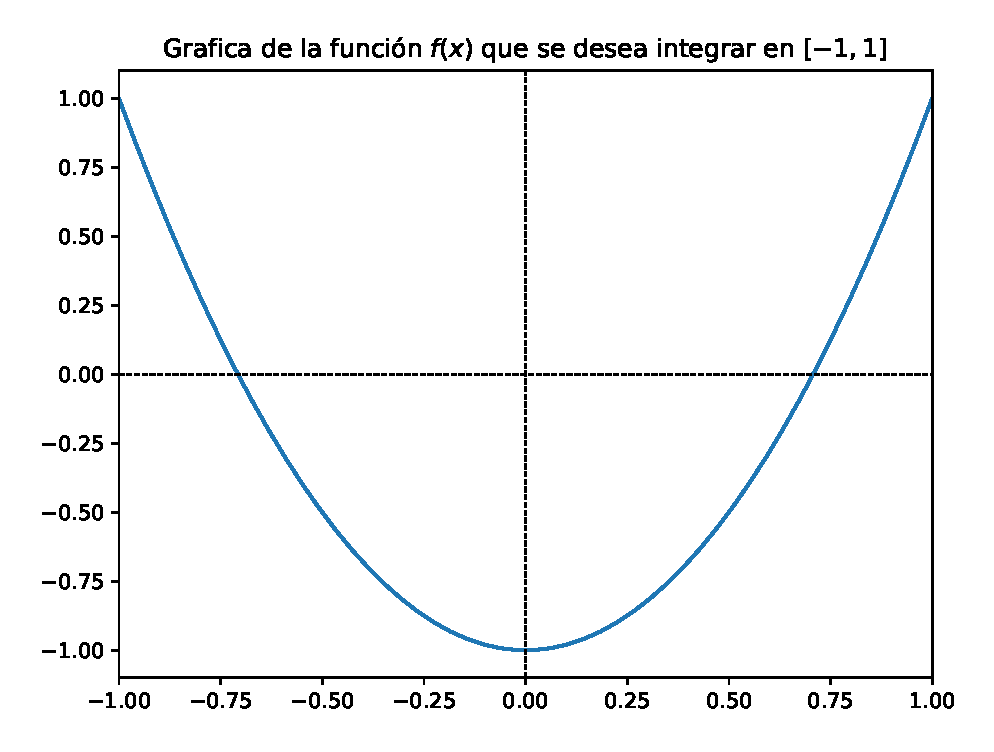
\includegraphics[scale=0.5]{Imagenes/integral_1_3_simpson.eps}
%     \caption{Queremos calcular el valor del área debajo de la curva.}
% \end{figure}
% \end{frame}
% \begin{frame}[allowframebreaks, fragile]
% \begin{lstlisting}[caption=Propuesta de código, style=FormattedNumber, basicstyle=\linespread{1.1}\ttfamily=\small, columns=fullflexible]
% def Simpson_13_(f, x_0_, xf, n):
   
%    n = n - n%2 # truncar al numero par mas cercano
%    print ('Para n= ' + str(n))
   
%    if n <= 0:
%       n = 1
   
%    h = (xf - x_0_)/n
%    x = x_0_
   
%    suma = 0
   
%    for j in range(int(n/2)):
%       suma += f () + 4. * f ( + h) + f ( + 2 * h)
%       x += 2 * h
%    return (h/3.) * suma
% \end{lstlisting}
% \end{frame}
% \begin{frame}[allowframebreaks, fragile]
% \begin{lstlisting}[caption=Solución al problema, style=FormattedNumber, basicstyle=\linespread{1.1}\ttfamily=\small, columns=fullflexible]
% def f ():
%     return cos(2 * acos(x))

% for i in range(1, 4):
%     print ('La integral I vale = ' + str(Simpson_13_(f, -1., 1., i * 2)) + '\n')
% \end{lstlisting}
% \end{frame}
% \begin{frame}[fragile]
% \frametitle{Solución en la terminal}
% \begin{verbatim}
% Para n = 2
% La integral I vale = -0.6666666666666666

% Para n = 4
% La integral I vale = -0.6666666666666665

% Para n = 6
% La integral I vale = -0.6666666666666667 
% \end{verbatim}
% \end{frame}


\end{document}